\chapter{Text automaton}
\label{chap-text-automaton}
\index{Automaton!of the text}
Natural languages contain much lexical ambiguity. The text automaton is an
effective and visual way of representing such ambiguity. Each sentence of a
text is represented by an automaton whose paths represent all possible
interpretations.

\bigskip
\noindent This chapter presents the concept of text automaton, the details of
their construction and the operations that can be applied, in particular ambiguity
removal and linearization. Since version 2.1, it is possible 
to search the text automaton for patterns (see section
\ref{section-locate-tfst}).


\section{Displaying text automaton} \index{Dictionaries!of the text}
The text automaton explicit all possible lexical interpretations of the
words. These different interpretations are the different entries presented in
the dictionary of the text.
Figure~\ref{fig-sentence-automaton} shows the automaton of the fourth
sentence of the text \textit{Ivanhoe}.

\begin{figure}[!ht]
\begin{center}
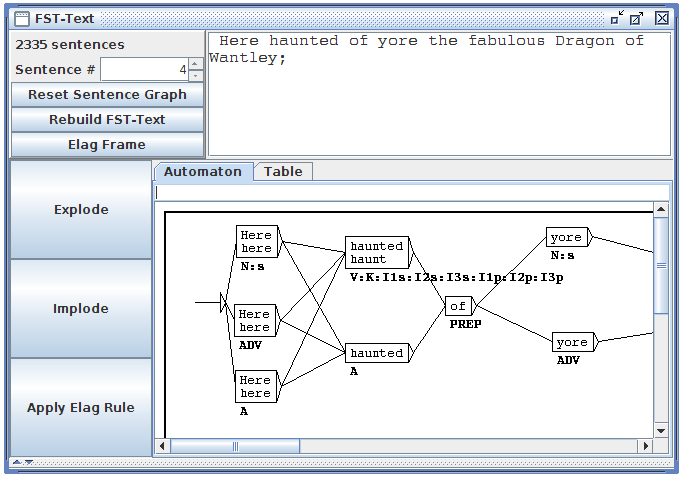
\includegraphics[width=15.5cm]{resources/img/fig7-1.png}
\caption{Sentence automaton example\label{fig-sentence-automaton}}
\end{center}
\end{figure}

\bigskip
\noindent You can see in Figure~\ref{fig-sentence-automaton}
that the word \verb+Here+ has three interpretations here (adjective, adverb and noun),
\verb+haunted+ two (adjective and verb), etc. All the possible combinations are
expressed because each interpretation of each word is connected to all the
interpretations of the following and preceding words.

\bigskip
\noindent In case of an overlap between a compound word and a sequence of simple words,
the automaton contains a path that is labeled by the compound word, parallel to
the paths that express the combinations of simple words. This is illustrated in
Figure~\ref{fig-overlap}, where the compound word
\texttt{courts of law} overlaps with a combination of simple words.

\begin{figure}[!ht]
\begin{center}
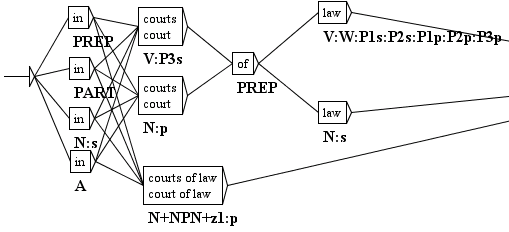
\includegraphics[width=12.5cm]{resources/img/fig7-2.png}
\caption{Overlap between a compound word and a combination of simple
words.\label{fig-overlap}}
\end{center}
\end{figure}

\bigskip
\noindent By construction, the text automaton does not contain any
loop. One says that the text automaton is \textit{acyclic}.\index{Automaton!acyclic}
\index{Acyclic automaton}

\bigskip
\noindent NOTE: The term ``text automaton'' is an abuse of language. In fact, there is an
automaton for each sentence of the text. Therefore, the combination of all these 
automata corresponds to the automaton
of the text. This is why we use the term ``text automaton'' even if this object
is not manipulated as a global automaton for practical reasons.

\section{Construction}
In order to construct the text automaton, open the text, then click on 
"Construct FST-Text..." in the menu "Text". One should first split the text into
sentences and  apply dictionaries. If sentence boundary detection
is not applied, the construction program will arbitrarily split the text in
sequences of 2000 lexical units instead of constructing one automaton per
sentence. If no dictionaries are applied, the text automaton that you
obtain will consist of only one path made up of unknown words per sentence.


\subsection{Construction rules for text automata}
\index{Granularity of dictionaries}\index{Dictionaries!granularity}\index{Degree of ambiguity}
Sentence automata are constructed from text dictionaries. The
resulting degree of ambiguity is therefore directly linked to the granularity of
the descriptions of dictionaries. From the sentence automaton
in figure~\ref{fig-ambiguity-of-which}, you can conclude that the word
\verb+which+ has been coded twice as a determiner in two subcategories of the
category \verb+DET+. This granularity of descriptions will not be of any use if
you are only interested in the grammatical category of this word. It is
therefore necessary to adapt the granularity of the dictionaries to the intended use.

\begin{figure}[!ht]
\begin{center}
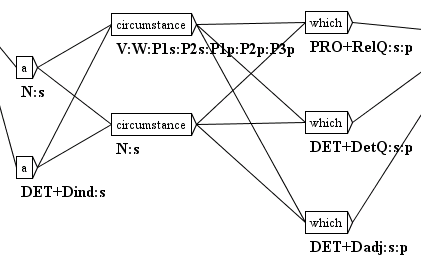
\includegraphics[width=10.6cm]{resources/img/fig7-3.png}
\caption{Double entry for \texttt{which} as a
determiner\label{fig-ambiguity-of-which}}
\end{center}
\end{figure}

\bigskip
\noindent For each lexical unit of the sentence, Unitex searches the
dictionary of the simple words of the text for all possible interpretations. Afterwards,
all combination of lexical units that have an interpretation in the dictionary
of the compound words of the text are taken into account. All the combinations
of these information constitute the sentence automaton.

\bigskip
\noindent NOTE: If the text contains lexical labels (\textit{e.g.}
\verb${out of date,.A+z1}$), these labels are reproduced identically in the
automaton without trying to decompose them.
\index{Lexical!labels}

\bigskip
\noindent In each box, the first line contains the inflected form found in the
text, and the second line contains the canonical form if it is different. The other
information is coded below the box.
(cf. section~\ref{section-displaying-sentence-automata}).

\bigskip
\noindent The spaces that separate the lexical units are not copied into the
automaton except for the spaces inside compound words.

\bigskip
\noindent The case of lexical units is retained. For example, if the word
\verb+Here+ is encountered, the capital letter is preserved (cf.
figure~\ref{fig-sentence-automaton}). This choice allows you to
keep this information during the transition to the text automaton,
which could be useful for applications where case is important as for
recognition of proper names.

\subsection{Normalization of ambiguous forms}
\index{Normalization!of the text automaton}\index{Normalization!of ambiguous
forms}
\index{Text!normalization of the automaton}
During construction of the automaton, it is possible to effect a normalization of
ambiguous forms by applying a normalization grammar. This grammar has to be
called \verb+Norm.fst2+ and must be placed in your personal folder, in the
subfolder \verb+/Graphs/Normalization+ of the desired language. The normalization
grammars for ambiguous forms are described in
section~\ref{section-normalizing-text-automataon}.

\bigskip
\noindent If a sequence of the text is recognized by the normalization grammar, all the
interpretations that are described by the grammar are inserted into the text
automaton.
Figure~\ref{fig-example-tfst-normalization-graph} shows
the part of the grammar used for the ambiguity of the sequence \verb+l'+ in French.

\begin{figure}[!ht]
\begin{center}
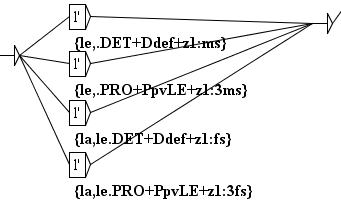
\includegraphics[width=8.6cm]{resources/img/fig7-4.png}
\caption{Normalization of the sequence \texttt{l'}\label{fig-example-tfst-normalization-graph}}
\end{center}
\end{figure}

\bigskip
\noindent If this grammar is applied to a French sentence containing the sequence
\verb+l'+, a sentence automaton that is similar to the one in
figure~\ref{fig-tfst-normalization-results} is obtained.

\begin{figure}[!ht]
\begin{center}
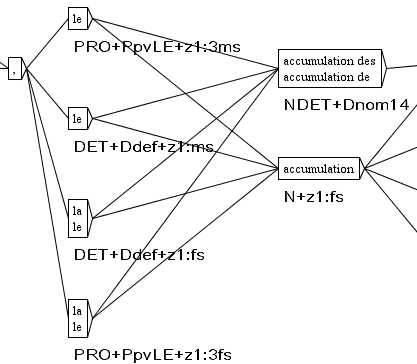
\includegraphics[width=10.2cm]{resources/img/fig7-5.png}
\caption{Automaton that has been normalized with the grammar of 
figure~\ref{fig-example-tfst-normalization-graph}\label{fig-tfst-normalization-results}}
\end{center}
\end{figure}

\bigskip
\noindent You can see that the four rules for rewriting the sequence \verb+l'+
have been applied, which has added four labels to the automaton. These labels are
not concurrent with the two preexisting paths for the sequence \verb+l'+,
because of the "keep best paths" heuristic (see section
\ref{section-keeping-best-paths}). The
normalization at the time of the construction of the automaton allows you to 
add paths to the automaton but not to remove ones. Removing paths will be
partially done by the "keep best paths" heuristic, if enabled. To go further,
you will need to use the ELAG disambiguation functionality.


\subsection{Normalization of clitical pronouns in Portuguese}
\label{section-portuguese-clitics}
\index{Clitics!normalization}\index{Normalization!of clitics in Portuguese}
\index{Portuguese!normalization of clitics}
In Portuguese, verbs in the future tense and in the conditional can be modified
by the insertion of one or two clitical pronouns between the root and the suffix
of the verb. For example, the sequence \textit{dir-me-\~ao} (\textit{they will
tell me}), corresponds to the complete verbal form \textit{dir\~ao}, associated
with the pronoun \textit{me}. In order to be able to manipulate this rewritten form,
it is necessary to introduce it into the text automaton in parallel to the
original form. Thus, the user can search one or the other form. The 
figures~\ref{fig-1285-not-normalized} and~\ref{fig-1285-normalized}  show the
automaton of a sentence after normalization of the clitics.


\begin{figure}[!ht]
\begin{center}
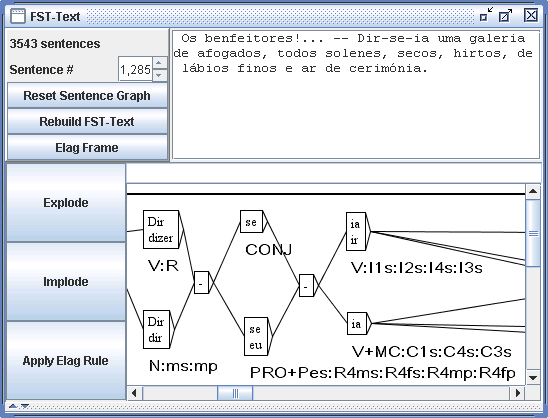
\includegraphics[width=11cm]{resources/img/fig7-6.png}
\caption{Non-normalized phrase automaton\label{fig-1285-not-normalized}}
\end{center}
\end{figure}
\begin{figure}[!ht]
\begin{center}
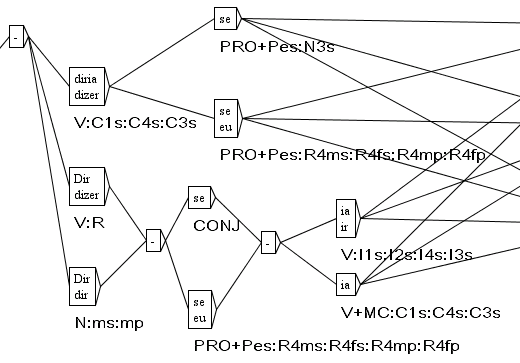
\includegraphics[width=11cm]{resources/img/fig7-7.png}
\caption{Normalized phrase automaton\label{fig-1285-normalized}}
\end{center}
\end{figure}
\clearpage

\index{External programs!\verb+Reconstrucao+}\index{\verb+Reconstrucao+}
\bigskip
\noindent The \verb+Reconstrucao+ program allows you to construct a
normalization grammar for these forms for each text dynamically. The grammar thus produced can then be
used for normalizing the text automaton. The configuration window of the
automaton construction suggests an option "Build clitic normalization grammar"
(cf. figure~\ref{fig-Txt2Tfst-configuration}). This option
automatically starts the construction of the normalization grammar, which is then
used to construct the text automaton, if you have selected the option "Apply the
Normalization grammar".



\subsection{Keeping the best paths}
\label{section-keeping-best-paths}
\index{Keeping the best paths}
An unknown word can perturb the text automaton by overlapping with a completely
labeled sequence. Thus, in the automaton of
figure~\ref{fig-unknown-word-ambiguity}, it can be seen that the
adverb

% do not remove this line jump
\noindent \verb+aujourd'hui+ overlaps with the unknown word \verb+aujourd+,
followed by an apostrophe and the past participle of the verb \verb+huir+.


\begin{figure}[!ht]
\begin{center}
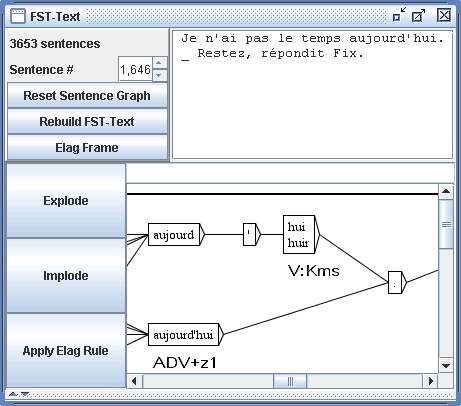
\includegraphics[width=11.6cm]{resources/img/fig7-8.png}
\caption{Ambiguity due to a sentence containing an unknown
word\label{fig-unknown-word-ambiguity}}
\end{center}
\end{figure}

\begin{figure}[!ht]
\begin{center}
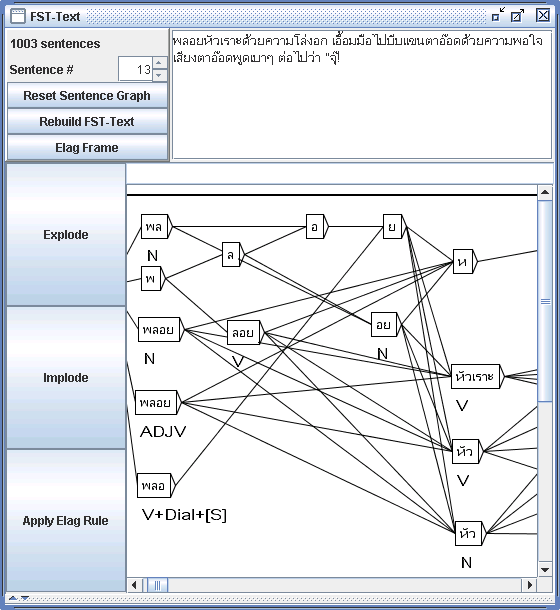
\includegraphics[width=14cm]{resources/img/fig7-9.png}
\caption{Automaton of a Thai
sentence\label{fig-thai-sentence-automaton}}
\end{center}
\end{figure}

\bigskip
\noindent This phenomenon can also take place in the treatment of certain Asian languages
like Thai. When words are not delimited, there is no other solution than to
consider all possible combinations, which causes the creation of numerous paths
carrying unknown words that are mixed with the labeled paths.
Figure~\ref{fig-thai-sentence-automaton} shows an example of such an automaton of a
Thai sentence.

\bigskip
\noindent It is possible to suppress parasite paths. You have to select the option "Clean
Text FST" in the configuration window for the construction of the text automaton
(cf. figure~\ref{fig-Txt2Tfst-configuration}).
This option indicates to the automaton construction program that it should clean
up each sentence automaton.

\begin{figure}[!ht]
\begin{center}
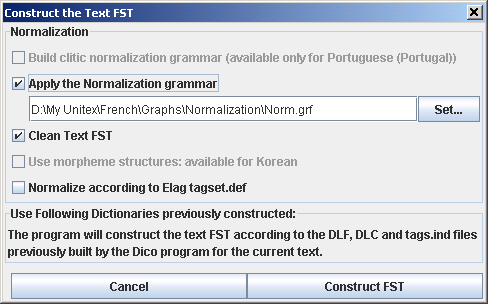
\includegraphics[width=14cm]{resources/img/fig7-10.png}
\caption{Configuration of the construction of the text automaton
\label{fig-Txt2Tfst-configuration}}
\end{center}
\end{figure}

\bigskip
\noindent This cleaning is carried out according to the following principle: if several
paths are concurrent in the automaton, the program keeps those that contain the
fewest unlabeled tokens. For instance, the compound adverb \verb+aujourd'hui+ is
preferred to the sequence made of \verb+aujourd+ followed by a quote and \verb+hui+, because
\verb+aujourd+ and the quote are both unlabeled tokens, while
the compound adverb path does not contain any unknown word.
Figure~\ref{fig-clean-thai-sentence-automaton} shows the automaton of
figure~\ref{fig-thai-sentence-automaton} after cleaning.

\begin{figure}[!ht]
\begin{center}
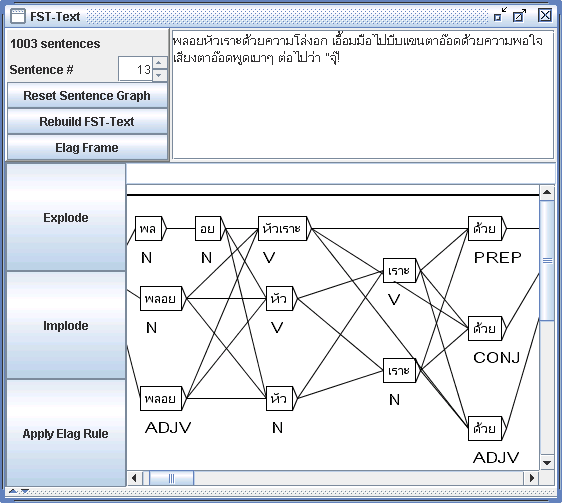
\includegraphics[width=10cm]{resources/img/fig7-11.png}
\caption{Automaton of
figure~\ref{fig-thai-sentence-automaton} after cleaning\label{fig-clean-thai-sentence-automaton}}
\end{center}
\end{figure}

\clearpage

\section{Resolving Lexical Ambiguities with ELAG}
\index{Ambiguity removal}\index{ELAG}
The ELAG program allows for applying grammars for ambiguity removal to the
text automaton. This powerful mechanism makes it possible to write rules on
independently from already existing rules. This chapter briefly presents the
grammar formalism used by ELAG and describes how the program works. For more
details, the reader may refer to \cite{elag-blanc-dister} and \cite{ELAG}.


\subsection{Grammars For Resolving Ambiguities}
\label{section-elag-grammars}
\index{Grammars!ambiguity removal}
The grammars used by ELAG have a special syntax. They consist of two parts which
we call the \textit{if} and \textit{then} parts. The \textit{if} part of an ELAG
grammar is divided in two parts which are divided by a box containing the \verb+<!>+ symbol. 
The \textit{then}
part is divided the same way using the \verb+<=>+ symbol. The meaning of a
grammar is the following: In the text automaton, if a path of the \textit{if}
part is recognized, then it must also be recognized by the \textit{then} part
of the grammar, or it will be withdrawn from the text automaton.

\begin{figure}[!ht]
\begin{center}
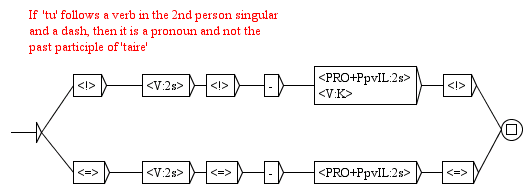
\includegraphics[width=13.1cm]{resources/img/fig7-12.png}
\caption{ELAG grammar \texttt{elag-tu.grf}\label{fig-elag-tu}}
\end{center}
\end{figure}

\bigskip
\noindent Figure~\ref{fig-elag-tu} shows an example of a grammar. The
\textit{if} part recognizes a verb in the 2$^{nd}$ person singular followed by a dash and
\verb+tu+, either as a pronoun, or as a past participle of the verb
\verb+taire+. The \textit{then} part imposes that \verb+tu+ is then regarded as
a pronoun. Figure~\ref{fig-applying-tu-grammar} shows the result of the
application of this grammar on the sentence "\textit{Feras-tu cela
bient\^ot$~$?}". One can see in the automaton at the bottom that the path
corresponding to \verb+tu+ past participle was eliminated.


\begin{figure}[!ht]
\begin{center}
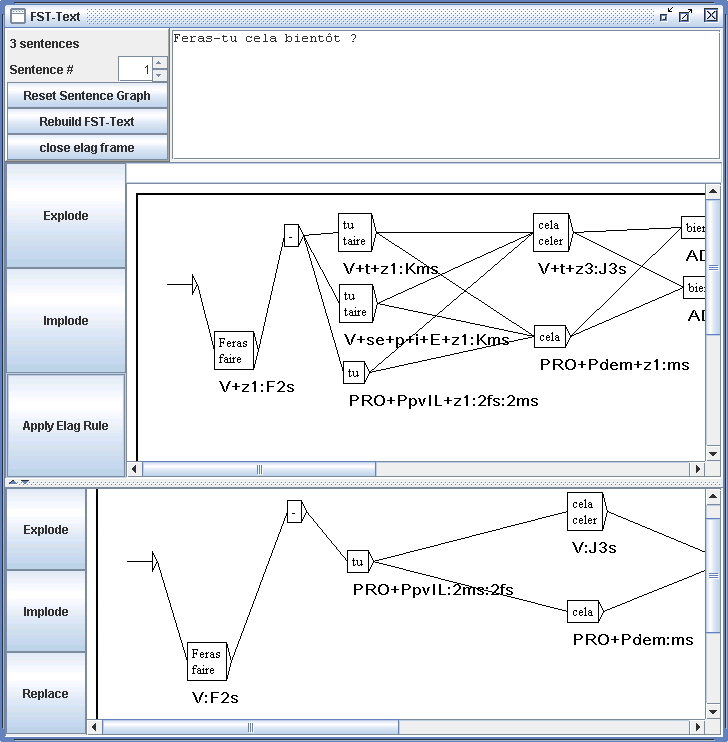
\includegraphics[width=14cm]{resources/img/fig7-13.png}
\caption{Result of applying the grammar in figure~\ref{fig-elag-tu}
\label{fig-applying-tu-grammar}}
\end{center}
\end{figure}

\begin{figure}[!ht]
\begin{center}
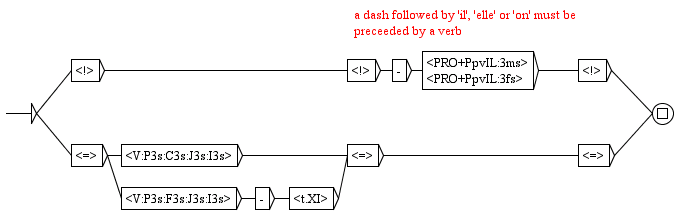
\includegraphics[width=14cm]{resources/img/fig7-14.png}
\caption{Use of the synchronization point\label{fig-synchronization-point}}
\end{center}
\end{figure}

\subsubsection{Synchronization point}
\index{Synchronization point}
The \textit{if} and \textit{then} parts of an ELAG grammar are divided into two
parts by \verb+<!>+ in the \textit{if} part, and \verb+<=>+ in the
\textit{then} part. These symbols form a \textit{synchronization point}.
This makes it possible to write rules in which the \textit{if} and
\textit{then} constraints are not necessarily aligned, as it is the
case for example in figure~\ref{fig-synchronization-point}. This grammar is
interpreted in the following way: if a dash is found followed by \verb+il+,
\verb+elle+ or \verb+on+, then this dash must be preceded by a verb, possibly
followed by \verb+-t+. So, if one considers the sentence of the
figure~\ref{fig-est-il} beginning with \textit{Est-il}, one can see 
that all non-verb interpretations of \verb+Est+ were removed.


\begin{figure}[!ht]
\begin{center}
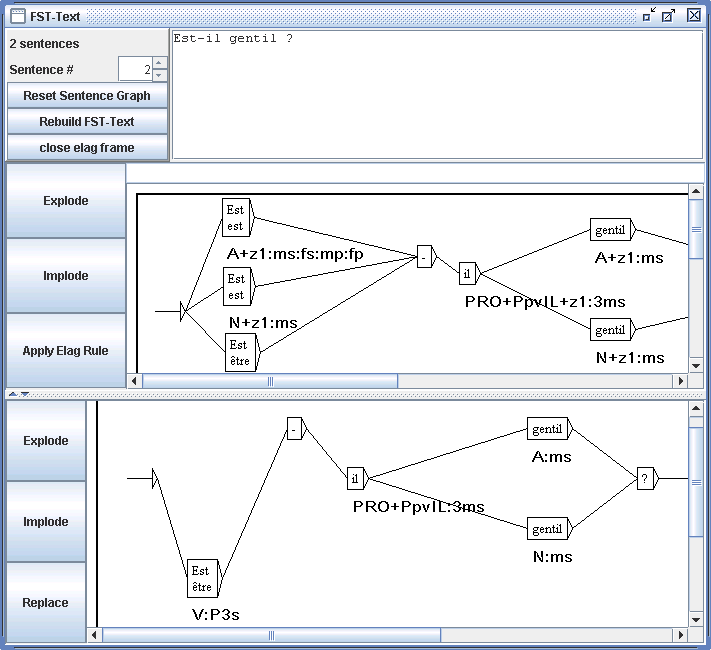
\includegraphics[width=14cm]{resources/img/fig7-15.png}
\caption{Result of the application of the grammar in
figure~\ref{fig-synchronization-point}\label{fig-est-il}}
\end{center}
\end{figure}

\subsection{Compiling ELAG Grammars}
\index{Compiling!ELAG grammars}
Before an ELAG grammar can be applied to a text automaton, the grammar must be
compiled in a  \verb+.rul+ file. \index{File!\verb+.rul+} This operation is
carried out via the "Elag Rules" command in the "Text" menu, which opens the
windows shown in figure~\ref{fig-elag-rules}.

\begin{figure}[!ht]
\begin{center}
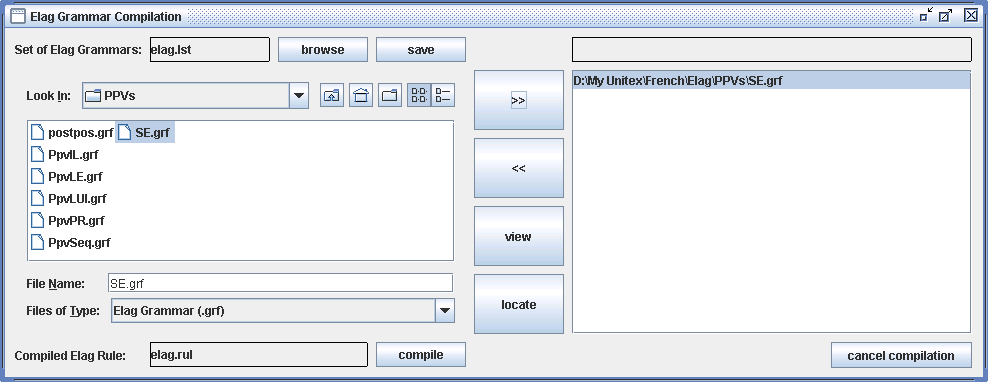
\includegraphics[width=15cm]{resources/img/fig7-16.png}
\caption{ELAG grammars compilation frame\label{fig-elag-rules}}
\end{center}
\end{figure}

\bigskip
\noindent If the frame on the right already contains grammars which you don't
wish to use, you can withdraw them with the "<<" button. Then select your
grammar(s) in the file explorer located in the left frame, and click on the
">>" button to add them to the list in the right frame. Then click on the
"Compile" button. This will launch the \verb+ElagComp+ program
\index{External programs!\verb+ElagComp+} which will compile the selected grammars and create a file named
\verb+elag.rul+ by default.\index{File!\verb+.rul+}

\bigskip
\noindent If you have selected grammars in the right frame, you can search patterns whith
them by clicking on the "Locate" button. This opens the window "Locate
Pattern" and automatically enters a graph name ending with
\verb+-conc.fst2+.\index{File!\verb+-conc.fst2+} This graphs corresponds to the
\textit{if} part of the grammar. You can thus obtain the occurrences of the
text to which the grammar will apply.

\bigskip
\noindent NOTE: The \verb+-conc.fst2+ file used to locate the \textit{if} part
of a grammar is automatically generated when ELAG grammars are compiled by means
of the "Compile" button. It is thus necessary to have your grammar
compiled before searching using the "Locate" button.


\subsection{Resolving Ambiguities}
\index{Resolving ambiguity}
Once you have compiled your grammar into an \verb+elag.rul+ file, you can apply
it to a text automaton. In the text automaton window, click on the "Apply Elag
Rule" button. A dialog box will appear which asks for the \verb+.rul+ file
to be used (see figure~\ref{fig-text-auto1}). The default file is
\verb+elag.rul+. This will launch the \verb+Elag+ program \index{External programs!\verb+Elag+} which
will try to resolve the ambiguity.

\begin{figure}[!ht]
\begin{center}
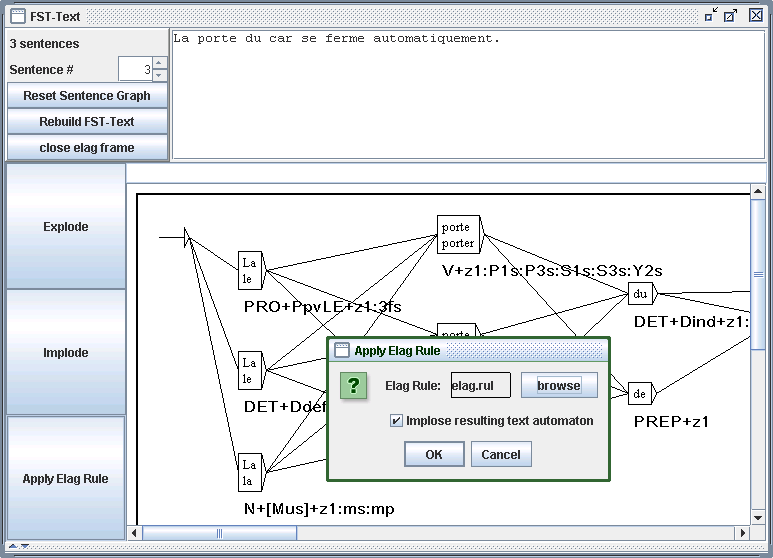
\includegraphics[width=12cm]{resources/img/fig7-17.png}
\caption{Text automaton frame \label{fig-text-auto1}}
\end{center}
\end{figure}

\bigskip
\noindent Once the program has finished you can view the resulting automaton by clicking on
the "Open Elag Frame" button. As you can see in figure~\ref{fig-text-auto2},
the windows is separated into two parts: The original text automaton can be seen
on the top, and the result at the bottom.

\begin{figure}[!h]
\begin{center}
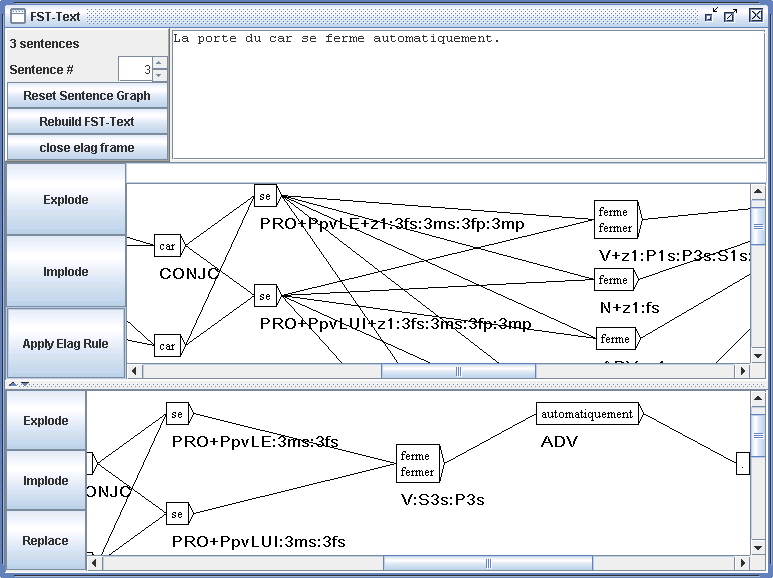
\includegraphics[width=12cm]{resources/img/fig7-18.png}
\caption{Splitted text automaton frame \label{fig-text-auto2}}
\end{center}
\end{figure}

\clearpage

\bigskip
\noindent Don't be surprised if the automaton shown at the bottom seems more complicated.
This results from the fact that factorized lexical entries\footnote{Entries which
gather several different inflectional interpretations, such as for example:

\texttt{\{se,.PRO+PpvLE:3ms:3fs:3mp:3fp\}}.}\index{Factorized lexical entries}
were exploded in order to treat each inflectional interpretation separately. To
refactorize these entries, click on the "Implode" button. Clicking on the
"Explode" button shows you an exploded view of the text automaton.

\bigskip
\noindent If you click on the "Replace" button, the resulting automaton will
become the new text automaton. Thus, if you use other grammars, they will apply to the
already partially disambiguated automaton, which makes it possible to accumulate
the effects of several grammars.


\subsection{Grammar collections}
\index{Grammars!collection}
It is possible to gather several ELAG grammars into a grammar collection in order
to compile and apply them in one step. The sets of ELAG grammars are described in
\verb+.lst+\index{File!\verb+.lst+} files. They are managed through the window
for compiling ELAG grammars (figure~\ref{fig-elag-rules}). The label on the top
left indicates the name of the current collection, by default \verb+elag.lst+.
The contents of this collection are displayed in the right part of the window.

\bigskip
\noindent To modify the name of the collection, click on the "Browse" button.
In the dialog box that appears, enter the \verb+.lst+ file name for the collection.

\bigskip
\noindent To add a grammar to the collection, select it in the file explorer in the left
frame, and click on the ">>" button. Once you have selected all your grammars,
compile them by clicking on the "Compile" button. This will create a
\verb+.rul+ file bearing the name indicated at the bottom right (the name of the file is
obtained by replacing \verb+.lst+ by \verb+.rul+).\index{File!\verb+.lst+}\index{File!\verb+.rul+}

\bigskip
\noindent You can now apply your grammar collection. As explained above, click on the
"Apply Elag Rule" button in the text automaton window. When the dialog asks for
the \verb+.rul+ file to use, click on the "Browse" button and select your
collection. The resulting automaton is identical to that which would have been
obtained by applying each grammar successively.

\subsection{Window For ELAG Processing}
\index{Window for ELAG Processing}
At the time of disambiguation, the \verb+Elag+ program
\index{External programs!\verb+Elag+} is launched in a processing window which displays the
messages printed by the program during its execution.

\bigskip
\noindent For example, when the text automaton contains symbols which do not correspond to
the set of ELAG labels (see the following section), a message indicates the
nature of the error. In the same way, when a sentence is rejected (all possible
analyses were eliminated by grammars), a message indicates the number of the
sentence. That makes it possible to locate the source of the problems quickly.


\subsubsection{Evaluation of ambiguity removal}
\index{Evaluation of the ambiguity rate}
\index{Ambiguity rate}
The evaluation of the ambiguity rate is not based solely on the average number
of interpretations per word. In order to get a more representative measure, the
system also takes into account the various combinations of words. While instances
of ambiguities are resolved, the \verb+Elag+ program calculates the number of
possible analyses in the text automaton before and after the modification (which
corresponds to the number of possible paths through the automaton). On the basis
of this value, the program computes the average ambiguity by sentence and word.
It is this last measure which is used to represent the ambiguity rate of the 
text, because it does not vary with the size of the corpus, nor with the number of
sentences within. The formula applied is:


\bigskip
\begin{center}
\textit{lexical ambiguity rate}$=exp^{\frac{log(number-of-paths)}{text-length}}$
\end{center}

\bigskip \noindent The relationship between the ambiguity rate before and
after applying the grammars gives a measure of their efficiency. All this
information is displayed in the ELAG processing window.


\subsection{Description of the tag sets}
\label{section-elag-tagset}
\index{ELAG tag sets}

The \verb+Elag+ and \verb+ElagComp+ programs 
\index{External programs!\verb+Elag+}
\index{External programs!\verb+ElagComp+} require a formal
description of the tag set to be used in dictionaries. This description
consists essentially of an enumeration of all the parts of speech present in the
dictionaries, with, for each of them, the list of syntactic and inflectional
codes compatible with it, and a description of their possible combinations. 
This description must be contained in a file called \verb$tagset.def$
and placed in your personal folder, in the \verb+Elag+ subfolder of
the desired language.


\subsubsection{\texttt{tagset.def} file}
\index{File!\verb$tagset.def$}
Here is an extract of the \verb$tagset.def$ file used for French.

\begin{verbatim}


NAME french

POS ADV
.

POS PRO
flex:
pers   = 1 2 3
genre  = m f
nombre = s p
discr:
subcat = Pind Pdem PpvIL PpvLUI PpvLE Ton PpvPR PronQ Dnom Pposs1s...
complete:
Pind     <genre> <nombre>
Pdem     <genre> <nombre>
Pposs1s  <genre> <nombre>
Pposs1p  <genre> <nombre>
Pposs2s  <genre> <nombre>
Pposs2p  <genre> <nombre>
Pposs3s  <genre> <nombre>
Pposs3p  <genre> <nombre>
PpvIL    <genre> <nombre> <pers>
PpvLE    <genre> <nombre> <pers>
PpvLUI   <genre> <nombre> <pers>      #
Ton      <genre> <nombre> <pers>      # lui, elle, moi
PpvPR                                 # en y
PronQ                                 # ou qui que quoi
Dnom                                  # rien
.

POS A ## adjectifs
flex:
genre  = m f
nombre = s p
cat:
gauche = g
droite = d
complete:
<genre> <nombre>
_  # pour {de bonne humeur,.A}, {au bord des larmes,.A} par exemple
.


POS V
flex:
temps  = C F I J K P S T W Y G X
pers   = 1 2 3
genre  = m f
nombre = s p
complete:
W
G
C <pers> <nombre>
F <pers> <nombre>
I <pers> <nombre>
J <pers> <nombre>
P <pers> <nombre>
S <pers> <nombre>
T <pers> <nombre>
X 1 s   # eusse dusse puisse fusse (-je)
Y 1 p
Y 2 <nombre>
K <genre> <nombre>
.
\end{verbatim}

\bigskip
\noindent The \verb$#$ symbol indicates that the remainder of the line is a
comment. A comment can appear at any place in the file. The file always starts with the word
\verb$NAME$, followed by an identifier (\texttt{french}, for example).
This is followed by the \verb$POS$ sections for each part of speech. Each section
describes the structure of the lexical tags of the lexical entries belonging to
the part of speech concerned. Each section is composed of 4 parts which are all
optional:

\begin{itemize}
  \item \verb$flex$\index{\verb$flex$}: this part enumerates the inflectional
  codes belonging to the grammatical category. For example, the codes
  \verb$1,2,3$ which indicate the person of the entry are relevant for pronouns
  but not for adjectives. Each line describes an inflectional attribute (gender,
  time, etc.) and is made up of the attribute name, followed by the \verb$=$
  character and the values which it can take. For example, the following line
  declares an attribute $pers$ being able to taking the values $1$, $2$ or $3$:

\begin{verbatim}
pers = 1 2 3
\end{verbatim}

\item \verb$cat$\index{\verb$cat$}: this part declares the syntactic and semantic
attributes which can be assigned to the entries belonging to the part of speech
concerned. Each line describes an attribute and the values which it can take. The
codes declared for the same attribute must be exclusive. In other words, an entry
cannot take more than one value for the same attribute.

On the other hand, all the tags in a given part of speech don't necessarily take
values for all the attribute of the part of speech. For example, to define the
attribute \verb$niveau_de_langue$ which can take the values \verb$z1$, \verb$z2$
and \verb$z3$, the following line can be written:


\begin{verbatim}
niveau_de_langue = z1 z2 z3
\end{verbatim}

but this attribute is not necessarily present in all words.

\item \verb$discr$\index{\verb$discr$}: this part consists of a declaration of a
unique attribute. The syntax is the same as in the \verb$cat$ part and the
attribute described here must not be repeated there. This part allows for
dividing the grammatical category in \textit{discriminating} sub categories in
which the entries have similar inflectional attributes. For pronouns for example,
a person feature is assigned to entries that are part of the personal pronoun sub
category but not to relative pronouns. These dependencies are described in the
\verb$complete$ part;

\item \verb$complete$\index{\verb$complete$}: this part describes the
inflectional part of the tags of the words in the current part of speech. Each
line describes a valid combination of inflectional codes by their discriminating
sub category (if such a category was declared). If an attribute name is specified
in angle brackets (\verb$<$ and \verb$>$), this signifies that any value of this
attribute may occur. It is possible as well to declare that an entry does not
take any inflectional feature by means of a line containing only the \verb$_$
character (underscore).\index{\verb$_$} So for example, if we consider that the
following lines extracted from the section describing the verbs:


\begin{verbatim}
W
K <genre> <nombre>
\end{verbatim}

They make it possible to declare that verbs in the infinitive (indicated by the
\verb$W$ code) do not have other inflectional features while the forms in the
past participle (\verb$K$ code) are also assigned a gender and a number.

\end{itemize}

\subsubsection{Description of the inflectional codes}
\index{Inflectional codes}
The principal function of the \verb$discr$ part is to divide a part of speech
into subcategories having similar inflectional behavior. These subcategories are
then used to facilitate writing the \verb$complete$ part.

\bigskip
\noindent For the legibility of the ELAG grammars, it is desirable that the
elements of the same subcategory all have the same inflectional behavior; in this case the
\verb$complete$ part is made up of only one line per subcategory.
Let us consider for example the following lines from the pronoun description:

\begin{verbatim}
Pdem  <genre> <nombre>
PpvIl <genre> <nombre> <pers>
PpvPr
\end{verbatim}

\bigskip
\noindent These lines mean:
\begin{itemize}
  \item all the demonstrative pronouns (\verb$PRO+Pdem>$) have only a gender and a number;
  \item clitic pronouns in the nominative (\verb$<PRO+PpvIl>$) are labelled
  grammatically in person, gender and number;
  \item the prepositional pronouns (\textit{en}, \textit{y}) do not have any
  inflectional feature.
\end{itemize}

\bigskip
\noindent All combinations of inflectional features and discriminant subcategories which
appear in the dictionaries must be described in the \verb$tagset.def$
file\index{File!\verb$tagset.def$}; otherwise, the information in the
corresponding entries will be discarded by ELAG.

\bigskip
\noindent If words of the same subcategory differ by their inflectional profile, it is
necessary to write several lines into the \verb$complete$ part. The disadvantage
of this method of description is that it becomes difficult to make the
distinction between such words in an ELAG grammar.

\bigskip
\noindent If one considers the description given by the previous example of a
\verb$tagset.def$ file, certain adjectives of French take a gender and a number,
whereas others to not have any inflectional feature. This allows for coding fixed
sequences like \textit{de bonne humeur} as adjective, on the basis of their
syntactic behavior.

\bigskip
\noindent Consider a French dictionary with such sequences as invariable adjectives without
inflectional features. The problem is that if one wants to refer exclusively to
this type of adjectives in a disambiguation grammar, the \verb$<A>$ symbol is not
appropriate, since it will recognize all adjectives. To circumvent this
difficulty, it is possible to deny an inflectional attribute by writing the
\verb$@$ character right before one of the possible values for this attribute.
Thus, the \verb$<A:@m@p>$ symbol recognizes all the adjectives which have neither
a gender nor a number. Using this operator, it is possible to write grammars like
those in figure~\ref{fig-NA}, which imposes agreement in gender and number
between a name and an adjective which suits\,\footnote{This grammar is not
completely correct, because it eliminates for example the correct analysis of the
sentence: \textit{J'ai re\c{c}u des coups de fil de ma m\`ere hallucinants.}}.
This grammar will preserve the correct analysis of sentences like: \textit{Les
personnes de bonne humeur m'insupportent}.

\bigskip
\noindent Is is however recommended to limit the use of the \verb$@$ operator, because it
harms the legibility of the grammars. It is preferable to distinguish the labels
which accept various inflectional combinations by means of discriminating
subcategories defined in the \verb$discr$ part.

\begin{figure}[!h]
\begin{center}
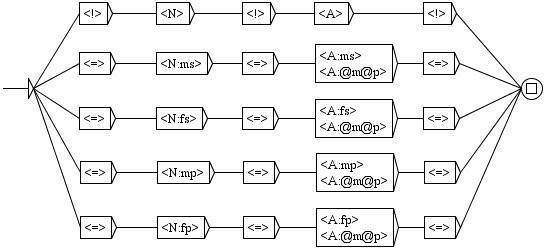
\includegraphics[width=12cm]{resources/img/fig7-19.png}
\caption{ELAG grammar that verifies gender and number agreement\label{fig-NA}}
\end{center}
\end{figure}

\subsubsection{Optional Codes}
The optional syntactic and semantic codes are declared in the \verb$cat$ part.
They can be used in ELAG grammars like other codes. The difference is that these
codes do not intervene to decide if a label must be rejected as an invalid one
while loading of the text autmaton.

\bigskip
\noindent In fact optional codes are independent of other codes, such as for example the
attribute of the language level (\verb$z1$, \verb$z2$ or \verb$z3$). In the same
manner as for inflectional codes, it is possible to deny an inflectional
attribute by writing the \verb$!$ character right before the name of the
attribute. Thus, with our example file, the \verb$<A!gauche:f>$ symbol recognizes
all adjectives in the feminine which do not have the \verb$gauche$
code\,\footnote{This code indicates that the adjective must appear on the left of
the nound to which it refers to, as is the case for \textit{bel}.}.

\bigskip
\noindent All codes which are not declared in the
\verb$tagset.def$\index{File!\verb$tagset.def$} file are discarded by ELAG. If a
dictionary entry contains such a code, ELAG will produce a warning and will
withdraw the code from the entry.

\bigskip
\noindent Consequently, if two concurrent entries differ in the original text automaton
only by undeclared codes, these entries will become indistinguishable by the
programs and will thus be unified into only one entry in the resulting automaton.

\bigskip
\noindent Thus, the set of labels described in the file \verb$tagset.def$ file is
compatible with the dictionaries distributed with Unitex, by factorizing words
which differ only by undeclared codes, and this independently of the applied
grammars.

\bigskip
\noindent For example, in the most complete version of the French dictionary, each
individual use of a verb is characterized by a reference to the lexicon grammar
table which contains it. We have considered until now that this information is
more relevant to syntax than to lexical analysis and we thus don't have
integrated them into the description of the tagset. They are thus automatically
eliminated at the time when the text automaton is loaded, which reduces the rate
of ambiguity.

\bigskip
\noindent In order to distinguish the effects bound to the tagset from those of the ELAG
grammars, it is advised to proceed to a preliminary stage of normalization of the
text automaton before applying disambiguation grammars to it. This normalization
is carried out by applying to the text automaton a grammar not imposing any
constraint, like that of figure~\ref{fig-elag-norm}. Note that this grammar is
normally present in the Unitex distribution and precompiled in the file
\verb+norm.rul+.\index{\verb+norm.rul+}\index{File!\verb+norm.rul+}

\begin{figure}[!h]
\begin{center}
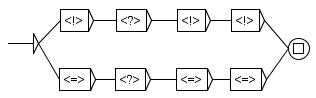
\includegraphics[width=9cm]{resources/img/fig7-20.png}
\caption{ELAG grammar without any constraint\label{fig-elag-norm}}
\end{center}
\end{figure}

\bigskip
\noindent The result of applying such a grammar is that the
original is cleaned of all the codes which either are not described in the \verb$tagset.def$
file\index{File!\verb$tagset.def$}, or do not conform to this description
(because of unknown grammatical categories or invalid combinations of
inflectional features). By then replacing the text automaton by this normalized
automaton, one can be sure that later modifications of the automaton will only be
effects of ELAG grammars.


\subsection{Grammar Optimization}
\index{Optimizing ELAG Grammars}
Compilation of ELAG grammars by the \verb+ElagComp+ program
\index{External programs!\verb+ElagComp+} consists in building an automaton
whose language is the set of the sequences of lexical tags (or lexical analyses of a sentence) which
are not accepted by the grammars. This task is complex and can take a lot of
time. It is however possible to appreciably speed it up by observing certain
principles at the time of writing gramars.

\subsubsection{Limiting the number of branches in the \textit{then} part}
It is recommended to limit the number of \textit{then} parts of a grammar to a
minimum. This can reduce considerably the compile time of a grammar. Generally, a grammar
having many \textit{then} parts can be rewritten with one or two \textit{then} parts, without a
loss of legibility. It is for example the case of the grammar in
figure~\ref{fig-NA-bad}, which imposes a constraint between a verb and the
pronoun which follows it.

\begin{figure}[!h]
\begin{center}
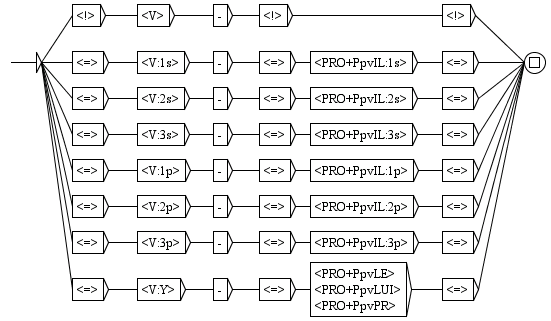
\includegraphics[width=15cm]{resources/img/fig7-21.png}
\caption{ELAG grammar checking verb-pronoun agreement\label{fig-NA-bad}}
\end{center}
\end{figure}

\bigskip
\noindent As one can see in figure~\ref{fig-NA-good}, one can write an
equivalent grammar by factorizing all the \textit{then} parts into only one. The two grammars will have
exactly the same effect on the text automaton, but the second one will be
compiled much more quickly.

\begin{figure}[!h]
\begin{center}
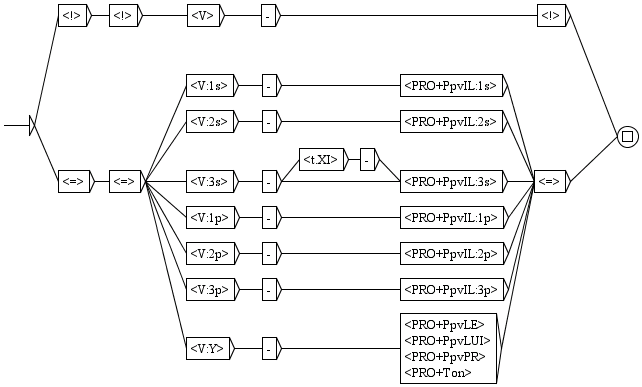
\includegraphics[width=15cm]{resources/img/fig7-22.png}
\caption{Optimized ELAG grammar checking verb-pronoun
agreement\label{fig-NA-good}}
\end{center}
\end{figure}


\subsubsection{Using lexical symbols}
\index{Lexical!symbols}

It is better to use lemmas only when it is necessary. That is particularly true
for some grammatical words, when their subcategories carry almost as much of
information as the lemmas themselves. In any case, it is recommended to specify
its syntactic, semantic and inflectional features as much as possible. For
example, with the dictionaries provided for French, it is preferable to replace
symbols like \verb$<je.PRO:1s>$, \verb$<je.PRO+PpvIL:1s>$ and \verb$<je.PRO>$
with the symbol \verb$<PRO+PpvI1:1s>$. Indeed, all these symbols are identical
insofar as they can recognize only the single entry of the dictionary
\verb${je,PRO+PpvIL:1ms:1fs}$. However, as the program does not deduce this
information automatically, if all these features are not specified, the program
will consider nonexisting labels such as \verb$<je.PRO:3p>$, 

% do not remove this line jump
\noindent \verb$<je.PRO+PronQ>$ etc. in vain.


\section{Linearizing text automaton with the tagger}
\label{section-linearization}
By default, the text automaton contains many paths of tags because of lexical ambiguity.
The linearization process consists in 
selecting a single path, a sequence of tags with one tag per token, and remove the others. 
The output of the process is a text automaton with a single path (see section \ref{section-linear-text}
for converting a linear automaton into linear text). The selection of a path depends on its score.
The path with the best score is chosen 
and the others are removed. The score of a path is calculated using a statistical model trained
on an annotated corpus. This model uses tagger data files generated by the TrainingTagger program 
(see section \ref{section-TrainingTagger}). 
For instance, you can see on Figure \ref{fig7-linearize2}, the original text automaton of the French sentence 
\textit{Les insectes nuisibles envahissent la maison}. The corresponding text automaton after linearization is 
shown on Figure \ref{fig7-linearize3}.

\begin{figure}[!ht]
\begin{center}
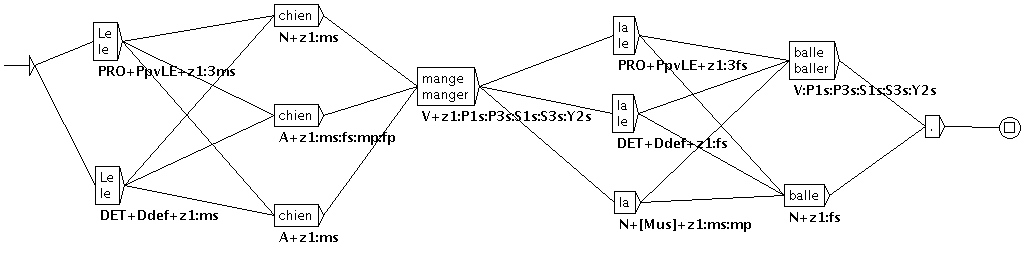
\includegraphics[width=16cm]{resources/img/fig7-linearize2.png}
\caption{Text automaton of \textit{Les insectes nuisibles envahissent la maison.}\label{fig7-linearize2}}
\end{center}
\end{figure}

\begin{figure}[!ht]
\begin{center}
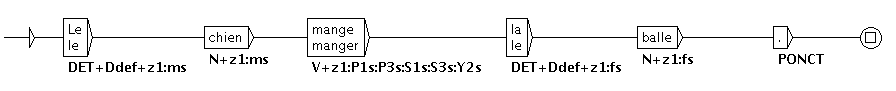
\includegraphics[width=16cm]{resources/img/fig7-linearize3.png}
\caption{Text automaton linearized\label{fig7-linearize3}}
\end{center}
\end{figure}

\subsection{Compatibility of the tagset}
\label{section-linearization-tagset}

The tagset of the tagger is identical to that of the training corpus or is a variant (see below). However, in order to use the tagger 
on a text automaton, one should pay attention to tagset and morphology. The tagset of the model must be identical to that of the text automaton. For example, if the statistical model has been computed with the tag \verb+DET+ for the word \verb+the+, 
the corresponding tag in the text automaton must be \verb+DET+. Unitex provides functionality to modify word forms in the text, for example to normalize \verb+doesn't+ into \verb+does not+.
Applying replacing or normalization graphs could cause some morphological modifications on words.
If such processing is applied to the text, it must have been applied to the training corpus as well. 
If these rules are not respected, the tagger might not be able to keep the good path from the text automaton.

\bigskip
\noindent The TrainingTagger program produces two variants of the tagger. The first one prunes transitions on the basis of 
grammatical, semantic, syntactic and inflectional codes (for example, \verb$the.DET+Ddef:s$ versus \verb$the.DET+Ddef:p$). 
The second one prunes transitions on the basis of grammatical, semantic and syntactic codes (\verb$that.DET+Ddem$ versus 
\newline \verb$that.PRO+Pdem$). This option makes the training quicker and inflectional features are not needed
for all applications.

\subsection{Use of the Tagger}
In order to linearize the text automaton, you have to select the option "Linearize with the Tagger" 
in the configuration window for the construction of the text automaton (cf. figure \ref{fig7-linearize1}). 
With this option, the program will linearize each sentence automaton. 
You must also select the tagger data file (with ".bin" extension) by clicking on the "Set" button.
Tagger data file suffixed by "morph" is the first variant of the tagger (with inflectional codes) and 
the one suffixed by "cat" is the second variant (without inflectional codes). 
If you want to use the "morph" data, you also need to click on "Normalize according to Elag 
tagset.def" (for more details, see section \ref{section-Tagger} about \verb+Tagger+ program).

\begin{figure}[!ht]
\begin{center}
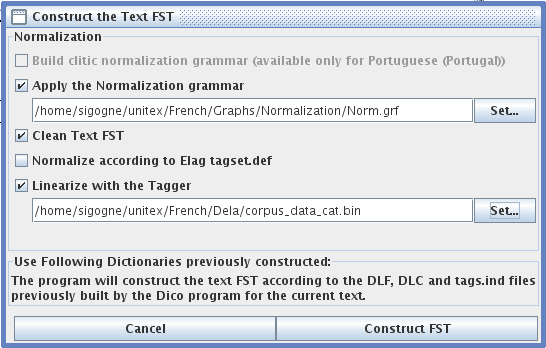
\includegraphics[width=13cm]{resources/img/fig7-linearize1.png}
\caption{Configuration of the linearization of the text automaton\label{fig7-linearize1}}
\end{center}
\end{figure}

\bigskip
\noindent For instance, the text automaton, shown on Figure \ref{fig7-linearize3}, is the output of linearization of the text automaton 
shown on Figure \ref{fig7-linearize2} with "cat" tagger data. 
Linearization of the automaton with "morph" tagger data is shown on Figure \ref{fig7-linearize4}.

\begin{figure}[!ht]
\begin{center}
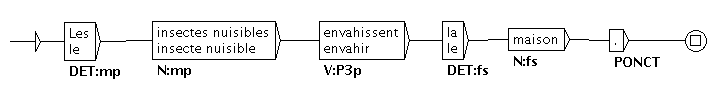
\includegraphics[width=16cm]{resources/img/fig7-linearize4.png}
\caption{Text automaton linearized with "morph" tagger data\label{fig7-linearize4}}
\end{center}
\end{figure}

\subsection{Creation of a new tagger}
In order to create a new tagger for your language, you need to launch the TrainingTagger program on your own annotated corpus.
The format of the annotated corpus is described in \ref{section-corpus-file}. As we discuss in Section \ref{section-linearization-tagset}, 
you need to pay attention on tagset and morphology. Before computing a statistical model, you have to decide which dictionaries and normalization
graphs you will use to construct the text automaton. And then, you will have to do modifications on the annotated corpus 
if word forms or tagset do not match completely. For example, if the normalization graph transforms the word \verb+jusqu'+ into \verb+jusque+,
 the corresponding word into the annotated corpus must be \verb+jusque+. 

\bigskip
\noindent A French tagger is distributed with Unitex. It has been created 
with an annotated corpus composed of tags without semantic and syntactic codes.



\section{Manipulation of text automata}

\subsection{Displaying sentence automata}
\label{section-displaying-sentence-automata}
As we have seen above, the text automaton is in fact the collection of the
sentence automata of a text. This structure can be represented using the format
\verb+.fst2+, also used for representing the compiled
grammars.\index{File!\verb+.fst2+} This format does not allow the system to
directly display the sentence automata. Instead, the system uses the
\verb+Fst2Grf+ program\index{\verb+Fst2Grf+}\index{External
programs!\verb+Fst2Grf+} to convert the sentence automaton into a graph that can
be displayed. This program is called automatically when you select a sentence  in
order to generate the corresponding \verb+.grf+ file.
\index{File!\verb+.grf+}

\bigskip
\noindent The generated \verb+.grf+ files are not interpreted in the same manner
as the \verb+.grf+ files that represent graphs constructed by the user. In fact,
in a normal graph, the lines of a box are separated by the \verb$+$ symbol. In
the graph of a sentence, each box represents either a lexical unit without a tag
or a dictionary entry enclosed by curly brackets. If the box only represents an
unlabeled lexical unit, this unit appears alone in the box. If the box represents
a dictionary entry, the inflected form is displayed, followed in another line by
the canonical form if it is different. The grammatical and inflectional
information is  displayed below the box as a transducer output.


\bigskip
\noindent Figure~\ref{fig-first-sentence-Ivanhoe} shows
the graph obtained for the first sentence of \textit{Ivanhoe}. The words \verb+Ivanhoe+,
\verb+Walter+ and \verb+Scott+ are considered unknown words. The word \verb+by+
corresponds to two entries in the dictionary. The word \verb+Sir+ corresponds to
two dictionary entries as well, but since the canonical form of these entries is
\verb+sir+, it is displayed because it differs from the inflected form by a lower
case letter.

\begin{figure}[!ht]
\begin{center}
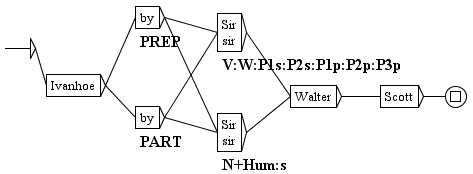
\includegraphics[width=11cm]{resources/img/fig7-23.png}
\caption{Automaton of the first sentence of \textit{Ivanhoe}\label{fig-first-sentence-Ivanhoe}}
\end{center}
\end{figure}

\subsection{Modifying the text automaton}
It is possible to manually modify the sentence automaton. You can add or erase
boxes or transitions. When a graph is modified, it is saved to the text file  
\verb+sentenceN.grf+, where $N$ represents the number of the sentence.

\bigskip
\noindent When you select a sentence, if a modified graph exists for this sentence, this
one is displayed. You can then reset the automaton of that sentence by clicking
on the botton "Reset Sentence Graph" (cf. 
figure~\ref{fig-modified-sentence-automaton}).

\begin{figure}[!ht]
\begin{center}
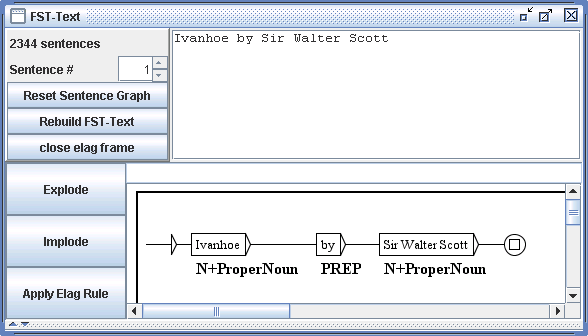
\includegraphics[width=15cm]{resources/img/fig7-24.png}
\caption{Modified sentence automaton\label{fig-modified-sentence-automaton}}
\end{center}
\end{figure}

\bigskip
\noindent During the construction of the text automaton, all the modified
sentence graphs in the text file are erased.

\bigskip
\noindent NOTE: After you reconstruct the text automaton, you can save your
manual modifications. In order to do that, click on the button "Rebuild
FST-Text". All sentences that have been modified are then replaced in the text
automaton by their modified versions. The new text automaton is then
automatically reloaded.

\subsubsection{Manually resolve Ambiguities}
The text automaton may contains many paths of tags because of lexical ambiguity. You can resolve ambiguities with ELAG Grammars or manually select the right paths for one or each graph of the sentence automaton.
To do so you can perform a right click on the box you want to keep when several boxes with different tags are proposed. The edges of the selected box will become more bold when the other boxes will appear grayed (see Figure~\ref{fig-manually-resolve-ambiguities}).

\begin{figure}[!ht]
\begin{center}
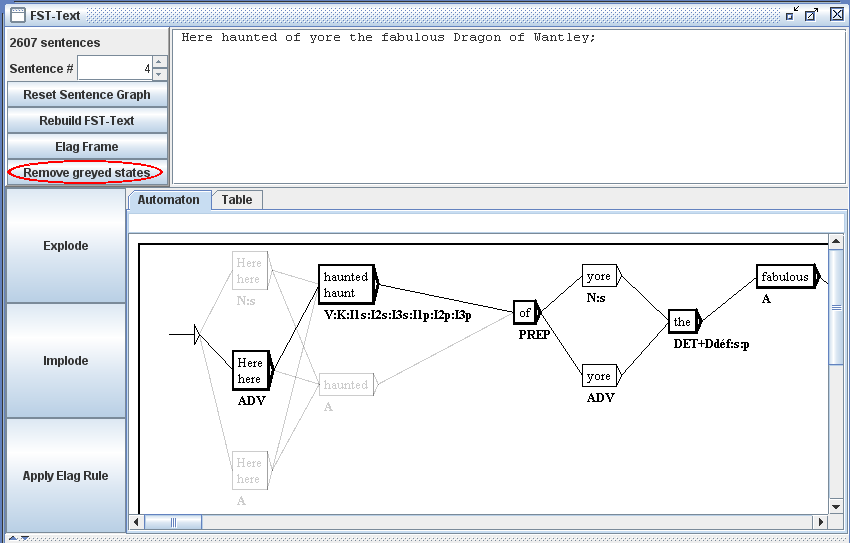
\includegraphics[width=15cm]{resources/img/fig7-24b.png}
\caption{Manually resolve ambiguities in sentence automaton\label{fig-manually-resolve-ambiguities}}
\end{center}
\end{figure} 

\bigskip
\noindent You can then click on the "Remove greyed states" button to keep only the selected boxes as in Figure~\ref{fig-removed-ambiguities}.
\begin{figure}[!ht]
\begin{center}
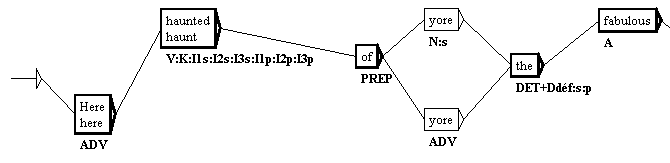
\includegraphics[width=11cm]{resources/img/fig7-24c.png}
\caption{Ambiguous boxes removed in sentence automaton\label{fig-removed-ambiguities}}
\end{center}
\end{figure}

\bigskip
\noindent 
\subsection{Display configuration}
Sentence automata are subject to the same presentation options as the
graphs. They use the same colors and fonts as well as the antialiasing effect. In
order to configure the appearance of the sentence automata, you  modify
the general configuration by clicking on "Preferences..." in the "Info" menu.
For further details, refer to section~\ref{section-display-fonts-colors}.

\bigskip
\noindent You can also print a sentence automaton by clicking on "Print..." in
the "FSGraph" menu or by pressing  <Ctrl+P>. Make sure that the printer's page
orientation is set to landscape mode. \index{Printing!a sentence automaton} To
configure this parameter, click on "Page Setup" in the
"FSGraph" menu.

\section{Converting the text automaton into linear text}
\label{section-linear-text}
\index{Text automaton!conversion into linear text}
If the text automaton does not contain any lexical ambiguity, it is possible to
build a text file corresponding to the unique path of the automaton. Go into the
"Text" menu and click on "Convert FST-Text to Text...". You can set the output
text file in the window as shown on Figure
\ref{fig-linearization-configuration}.

\begin{figure}[!ht]
\begin{center}
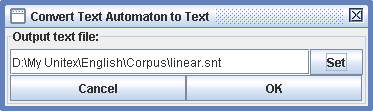
\includegraphics[width=10cm]{resources/img/fig7-25.png}
\caption{Setting output file for linearization of the text automaton\label{fig-linearization-configuration}}
\end{center}
\end{figure}

\bigskip
\noindent If the automaton is not linear, an error message will give you the number of
the first sentence that contain ambiguity. Otherwise, the \verb+Tfst2Unambig+ program
will build the output file according to the following rules:

\index{External programs!\verb+Tfst2Unambig+}\index{\verb+Tfst2Unambig+}
\begin{itemize}
  \item the output file contains one line per sentence;
  \item every line but the last is ended by \verb+{S}+;
  \item for each box, the program writes its content followed by a space.
\end{itemize}

\begin{figure}[!ht]
\begin{center}
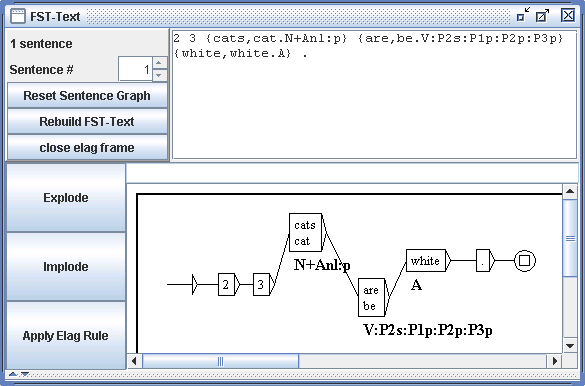
\includegraphics[width=12cm]{resources/img/fig7-26.png}
\caption{Example of a linear text automaton\label{fig-linear-automaton}}
\end{center}
\end{figure}

\bigskip
\noindent NOTE: correcting spaces in the output text can only be done manually. If the
original text is the one of the text automaton shown on Figure \ref{fig-linear-automaton},
the output text will be:

\begin{verbatim}
2 3 {cats,cat.N+Anl:p} {are,be.V:P2s:P1p:P2p:P3p} {white,white.A} .
\end{verbatim}


\section{Searching patterns in the text automaton}
\label{section-locate-tfst}
With the \verb+LocateTfst+ program, Unitex can perform search operations on the
text automaton. The main advantages are that you can:
\begin{itemize}
    \item benefit from ambiguity removal;
    \item benefit from the application of normalization grammar (see below);
    \item work at several morphological levels (multi-word units, simple words,
    morphemes). This is particularly interesting since you can now
    easily manipulate agglutinative languages like Korean (for Korean, see
    section \ref{section-korean}).
   
\end{itemize}

 
\bigskip
\noindent The rules are very similar to the ones that apply to classical
searches with \verb+Locate+. Here are the differences:

\begin{itemize}
    \item you cannot capture sequences with variables inside right contexts, as
    it is possible with \verb+Locate+ (see Figure \ref{fig-context6},
    page \pageref{fig-context6})
    
    \item you cannot match things that are not in the text automaton: 
    if the text automaton only contains a compound word tag and not
    its concurrent simple word tags, you won't be able to match simple words.
    For instance, in the sentence automaton shown on Figure
    \ref{fig7-locatetfst1}, it is not possible to match \verb+soixante+
    or \verb+huit+, since there are no such paths.
    
\begin{figure}[!ht]
\begin{center}
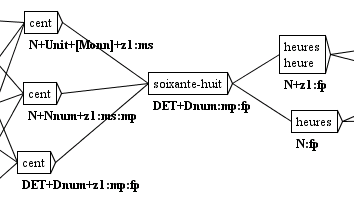
\includegraphics[width=9cm]{resources/img/fig7-locatetfst1.png}
\caption{Sentence automaton that cannot match with
pattern \textit{huit}\label{fig7-locatetfst1}}
\end{center}
\end{figure}

    \item matched sequences can differ from sequences that will appear in
    concordances. In fact, the text automaton may contain tags that do not
    correspond to the raw input text, in particular when a normalization grammar
    has been applied. For instance, if you look for the pattern \verb+<le.DET>+
    in \textit{80jours}'s text automaton, you will obtain 7703 matches, while
    \verb+Locate+ only finds 5763 matches. This is because some words have been normalized,
    like \verb+au+ $\rightarrow$ \texttt{\`a le} or \verb+du+ $\rightarrow$
    \verb+de le+. So, when you look for \verb+<le.DET>+, \verb+LocateTfst+
    matches those tags that were added to the text automaton by the
    normalization grammar, and \verb+Concord+ uses the original sequence in the
    text to produce the concordance file, as shown on Figure
    \ref{fig7-locatetfst2}.

\begin{figure}[!ht]
\begin{center}
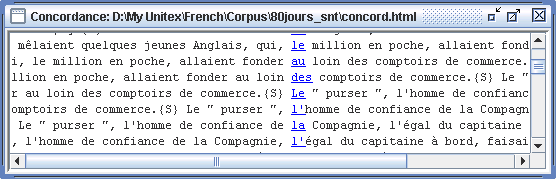
\includegraphics[width=14cm]{resources/img/fig7-locatetfst2.png}
\caption{A surprising concordance for pattern
\texttt{<le.DET>}\label{fig7-locatetfst2}}
\end{center}
\end{figure}

    \item \verb+<TOKEN>+\index{\verb+<TOKEN>+} does not match tokens as defined
    in \verb+tokens.txt+\index{\verb+tokens.txt+}. It matches any tag of the
    text automaton. Matched tags can be either longer than text tokens if they
    are compound word tags, or even shorter, if the text automaton contains 
    morphological analysis like \verb+un+ as shown on 
    Figure \ref{morphoB}, page \pageref{morphoB}.
	




\end{itemize}


\section{Table display}
\label{section-table-display}
Sentence automata can be displayed in a table format. To do that, you just have to select
the "Table" tab in the text automaton frame. You will then see a table as shown on Figure
\ref{fig7-table1}.


\begin{figure}[!ht]
\begin{center}
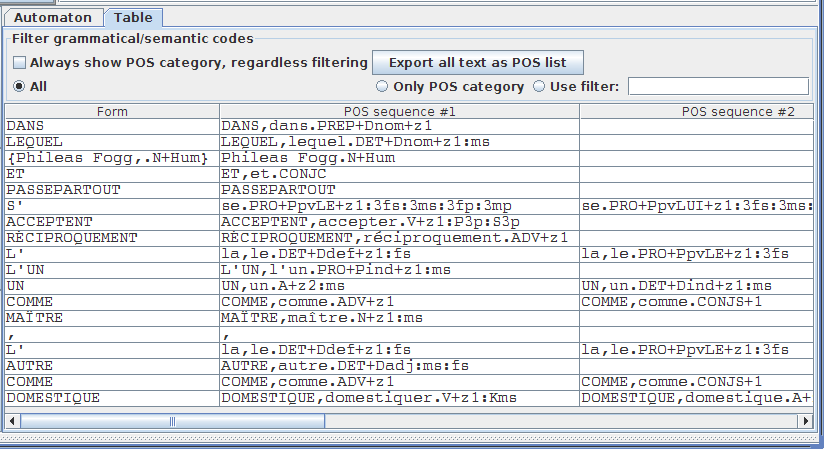
\includegraphics[width=14.5cm]{resources/img/fig7-table1.png}
\caption{Table display\label{fig7-table1}}
\end{center}
\end{figure}

\bigskip
\noindent This table is not fully equivalent to the sentence automaton, since it only
displays all possible POS for each simple or multiple word unit. It should be considered
as an approximate compact view of information contained in the automaton. You can also filter
grammatical/semantic codes to be displayed. Select "All" and you will see all codes. Select
"Only POS category" and only first codes (supposed to represent the POS category) will be displayed.
If you select "Use filter" and set a regular expression $X$, codes that do not contain something 
matched by $X$ will be discarded. Any POSIX regular expression is accepted as filter. Check 
"Always show POS category", and as said, the POS category will be kept even if not matched by the filter,
if any. For instance, Figure \ref{fig7-table2} shows a filtering result, obtained with the filter
\verb+^[A-Z]+ that matches any code starting with an uppercase letter, thus discarding codes like
\verb+z1+.

\begin{figure}[!ht]
\begin{center}
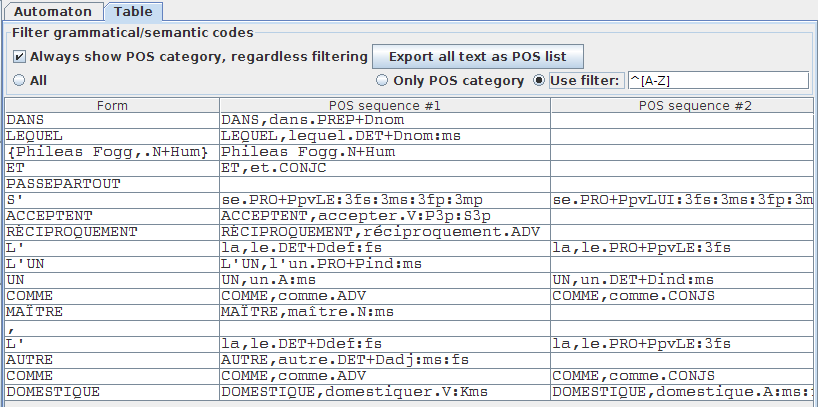
\includegraphics[width=14.5cm]{resources/img/fig7-table2.png}
\caption{Filtered table display\label{fig7-table2}}
\end{center}
\end{figure}
      
\bigskip
\noindent The "Export all text as POS list" button can be used to export this table display
of the whole text automaton as a text file following a special format. Currently, it is
only an experimental feature that may change in the future. Here is an example of output:

\begin{verbatim}
(Je/N:ms:mp)|(Je/PRO/PpvIL:1fs:1ms) (suis/V:P1s)|(suis/V:Y2s:P2s:P1s) 
M/N:mp:ms . Mdiba (de/DET/Dind:fp:mp:fs:ms)|(de/PREP)|(de/PREP/z1
+de la/DET/Dind/z1:fs)|(de/PREP/z1+des/DET/Dind/z1:mp:fp)|(de/PREP/z1
+du/DET/Dind/z1:ms)|(de la/DET/Dind/z1:fs)|(des/DET/Dind/z1:mp:fp)|
(du/DET/Dind/z1:ms) LG - ville/N:fs . {S}
\end{verbatim}



\section{The special case of Korean}
\label{section-korean}
Korean is an agglutinative language that has a very special morphological
system: words are made of Hangul syllabic characters, but one Hangul character
corresponds to several Jamo alphabetic characters. For instance, you can see on
Figure \ref{fig7-korean1} two examples of Hangul characters followed by their
equivalent Jamo letter sequences.

\begin{figure}[!ht]
\begin{center}

\includegraphics[width=4.5cm]{resources/img/fig7-korean1.png}
\caption{Hangul characters and their equivalent Jamo
sequences\label{fig7-korean1}}
\end{center}
\end{figure}

\noindent Moreover, morphemes do not correspond necessarily to Hangul
characters. For instance, Figure \ref{fig7-korean2} shows that a given token
(shown in green) must be analyzed as a combination of two elements: a verb and
a modifier. The point is that the modifier is only made of one Jamo letter that
combines with the last Hangul character of the verb in order to give the last
Hangul character of the whole word (in green). The green tokens correspond to
untagged tokens. Untagged tokens are not highlighted in green for other
languages.

\begin{figure}[!ht]
\begin{center}
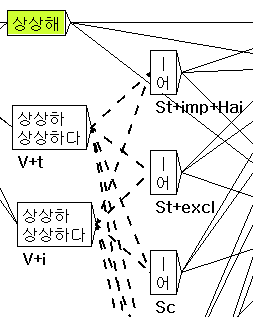
\includegraphics[width=6cm]{resources/img/fig7-korean2.png}
\caption{Decomposition of a Hangul character\label{fig7-korean2}}
\end{center}
\end{figure}

\bigskip
\noindent As a consequence, it can be convenient for Korean users to write
grammars with mixes of Hangul and Jamo characters. Thus, a grammar like the one shown on
Figure \ref{fig7-korean3} will match sequences like the one shown Figure 
\ref{fig7-korean4}.

\begin{figure}[!ht]
\begin{center}
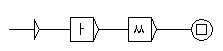
\includegraphics[width=5.5cm]{resources/img/fig7-korean3.png}
\caption{A grammar with two Jamo letters\label{fig7-korean3}}
\end{center}
\end{figure}

\begin{figure}[!ht]
\begin{center}
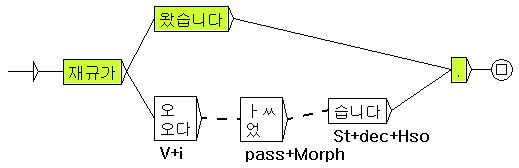
\includegraphics[width=13cm]{resources/img/fig7-korean4.png}
\caption{Sentence automaton matched by grammar of
Figure \ref{fig7-korean3}\label{fig7-korean4}}
\end{center}
\end{figure}

\bigskip
\noindent REMARKS: 
\begin{enumerate}
    \item Jamo letters are not in the Korean alphabet file
    (\verb+Alphabet.txt+). DO NOT ADD THEM TO THIS FILE, because it
    would induce dysfunctions in programs.\index{Alphabet!Korean}
    
    \item This alphabet file contains equivalences between some Chinese
    characters and some Hangul ones. In practice, if a grammar contains a
    Chinese character that has such an equivalent Hangul, it will match this
    Hangul in the text automaton. For instance, the grammar shown on Figure
    \ref{fig7-korean5} will match the sentence of Figure \ref{fig7-korean4},
    because the Korean alphabet file contains an equivalence for that
    character, as shown on Figure \ref{fig7-korean6}.\index{Chinese characters}
\end{enumerate}

\begin{figure}[!ht]
\begin{center}
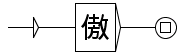
\includegraphics[width=5cm]{resources/img/fig7-korean5.png}
\caption{A grammar with a Chinese character\label{fig7-korean5}}
\end{center}
\end{figure}

\begin{figure}[!ht]
\begin{center}
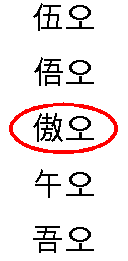
\includegraphics[width=3.5cm]{resources/img/fig7-korean6.png}
\caption{Extract of Korean alphabet file\label{fig7-korean6}}
\end{center}
\end{figure}